\documentclass[10pt,conference,letterpaper]{IEEEtran}
%\usepackage{amsmath,epsfig,multirow,color,latexsym}
\usepackage{graphicx}
\usepackage{subfigure}
\newtheorem{defi}{Definition}  % 在 preamble 區先定義好環境名稱
\usepackage{listings}
\usepackage{amssymb}
\usepackage{comment}
\usepackage[ruled,linesnumbered,noend]{algorithm2e}
\newcommand\mycommfont[1]{\footnotesize{#1}}
\SetCommentSty{mycommfont}
\usepackage{textcomp}
\usepackage{multirow}


\graphicspath{{figure/}}

\begin{document}
\title{KSTR: Keyword-aware Skyline Travel Route Recommendation}

\author{
\IEEEauthorblockN{Yu-Ting Wen\IEEEauthorrefmark{1},
Kae-Jer Cho\IEEEauthorrefmark{1},
Wen-Chih Peng\IEEEauthorrefmark{1},
Jinyoung Yeo\IEEEauthorrefmark{2},
Seung-won Hwang\IEEEauthorrefmark{3}
}
\IEEEauthorblockA{\IEEEauthorrefmark{1}National Chiao Tung University, Taiwan}
\IEEEauthorblockA{\IEEEauthorrefmark{2}Pohang University of Science and Technology, Republic of Korea}
\IEEEauthorblockA{\IEEEauthorrefmark{3}Yonsei University, Republic of Korea}
{\{ytwen,kjcho13,wcpeng\}@cs.nctu.edu.tw,jinyeo@postech.ac.kr,seungwonh@yonsei.ac.kr}
}

\maketitle

\begin{abstract}
With the popularity of social media (e.g., Facebook and Flicker), users could easily share their check-in records and photos during their trips. In view of the huge amount of check-in data and photos in social media, we intend to discover travel experiences to facilitate trip planning. Prior works have been elaborated on mining and ranking existing travel routes from check-in data. We observe that when planning a trip, users may have some keywords about preference on his/her trips. Moreover, a diverse set of travel routes is needed. To provide a diverse set of travel routes, we claim that more features of Places of Interests (POIs) should be extracted. Therefore, in this paper, we propose a Keyword-aware Skyline Travel Route (\textit{KSTR}) framework that use knowledge extraction from historical mobility records and the user's social interactions. Explicitly, we model the ``Where, When, Who'' issues by featurizing the geographical mobility pattern, temporal influence and social influence. Then we propose a keyword extraction module to classify the POI-related tags automatically into different types, for effective matching with query keywords. We further design a route reconstruction algorithm to construct route candidates that fulfill the query inputs. To provide diverse query results, we explore Skyline concepts to rank routes. To evaluate the effectiveness and efficiency of the proposed algorithms, we have conducted extensive experiments on real location-based social network datasets, and the experimental results show that \textit{KSTR} does indeed demonstrate good performance compared to state-of-the-art works. 
\end{abstract}

\section{Introduction}
Location-based social network services allow users to perform check-in and share their check-in data with their friends. In particular, when a user is traveling, the check-in data are in fact a travel trajectory with some photos and tag information. As a result, a massive number of trajectories are generated, which play an essential role in many well-established research areas, such as mobility prediction, urban planning and traffic management. In this paper, we focus on trip planning and intend to discover travel experiences from shared data in location-based social networks. To facilitate trip planning, the prior works in \cite{SIGMOD2010}\cite{hsieh2014mining}\cite{ICPADS2007}\cite{skyline2014}\cite{WWW2009} provide an interface in which a user could submit the query region and the total travel time. In contrast, we consider a scenario where users specify their preferences with keywords. For example, when planning a trip in Sydney, one would have ``Opera House''. As such, we extend the input of trip planning by exploring possible keywords issued by users. However, the query results of existing travel route recommendation services usually rank the trajectories simply by the popularity or the number of uploads of trajectories. 

For such ranking, existing works~\cite{yuan2014graph}\cite{ye2011exploiting}\cite{ytwen2014} derive a scoring function, and each trajectory will have one score according to its features (e.g., the number of Places of Interest, the popularity of places). Usually, the query results will have similar trajectories. In contrast, this work considers the diversity of results, as high scoring trajectories are often too similar to each other. Our goal is to retrieve a greater diversity of trajectories based on the travel factors considered.

 % Typically, a trajectory is a sequence of geo-locations with time-stamps, and a travel route may pass through a sequence of places of interest (POIs). Obviously, users would like to acquire travel routes that contains a set of POIs instead of individual ones. Note that every POI has its' proper visiting time. For example, people would like to go to night market in the night because there has a lot of vendors and people can enjoy their shopping and food travel. On the contrary, night market may have no venders and nothing interesting if people visit it in the day time. Furthermore, users may have some personalized requirements like must-visit POI(s) to be added into their trip plan. For instance, Tim wants to have a one day trip in Melbourne and he want to visit Federation Square. It would be helpful if a travel route recommendation system is able to recommend trips that contain Federation Square and some nearby interesting regions in Melbourne. Addition information can also be explored from geo-social network to find out influential friends, e.g., assume Tim always refer Kelly for travel tips, Tim would probably be interest in the travel itinerary Kelly has. % There are many representative work includes trajectory search frameworks \cite{SIGMOD2010,hsieh2014mining,ICPADS2007,skyline2014,WWW2009} mining knowledge form trajectories \cite{yuan2014graph,ye2011exploiting,ytwen2014}, and efficient search algorithms \cite{SIGMOD2010,ICDE2013,cao2012keyword} are proposed in these years. 

\begin{figure}[t]
\centering
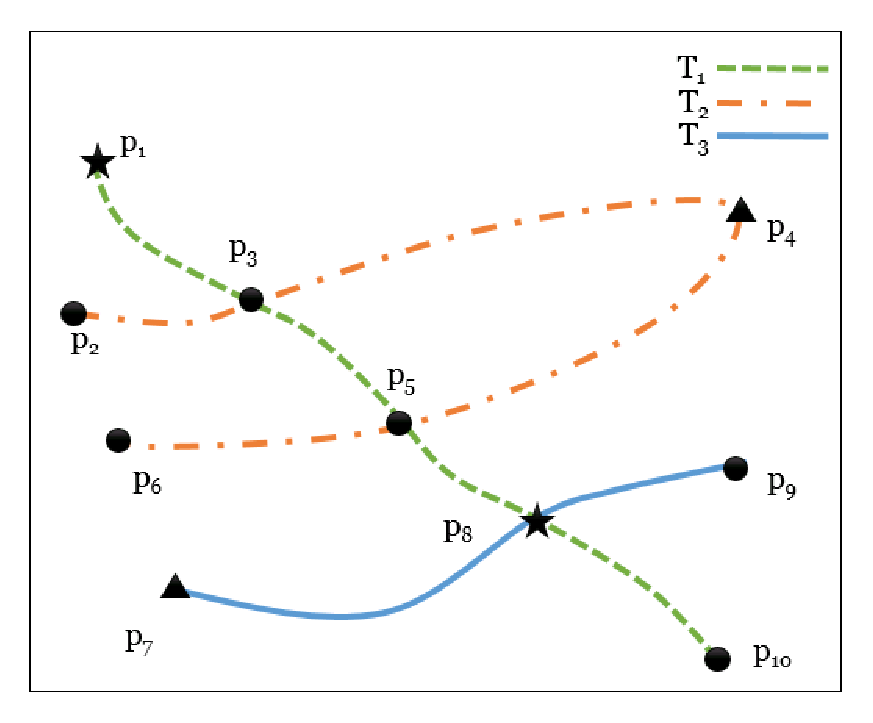
\includegraphics[width=6cm]{intro_example.eps}
\caption{Keyword-aware travel routes query running example.}
\label{fig:running_example}
\end{figure}

\begin{table}[t]
 \centering
 \caption{Example of trajectory dataset}
 \begin{footnotesize}
 \begin{tabular}{|c|l|l|l|l|l|} \hline
 Tid & Uid & Pid & keyword & time & POI score vector\\ \hline
 $T_{1}$ & $u_{1}$ & $p_{1}$ & Opera House & 10:00 & (0.04, 0.2) \\ \hline
 $T_{1}$ & $u_{1}$ & $p_{3}$ & Bar & 12:00 & (0.25, 0.2) \\ \hline
 $T_{1}$ & $u_{1}$ & $p_{5}$ & Bar & 15:30 & (0.2, 0.8) \\ \hline
 $T_{1}$ & $u_{1}$ & $p_{8}$ & Opera House & 17:30 & (0.04, 0.3) \\ \hline
 $T_{1}$ & $u_{1}$ & $p_{10}$ & Bar & 19:00 & (0.04, 0.2) \\ \hline
 $T_{2}$ & $u_{2}$ & $p_{2}$ & Bar & 10:30 & (0.02, 0.2) \\ \hline
 $T_{2}$ & $u_{2}$ & $p_{3}$ & Bar & 12:30 & (0.25, 0.2) \\ \hline
 $T_{2}$ & $u_{2}$ & $p_{4}$ & Sunset & 17:00 & (0.05, 0.2) \\ \hline
 $T_{2}$ & $u_{2}$ & $p_{5}$ & Bar & 19:00 & (0.2, 0.8) \\ \hline
 $T_{2}$ & $u_{2}$ & $p_{6}$ & Bar & 19:30 & (0.25, 0.8) \\ \hline
 $T_{3}$ & $u_{3}$ & $p_{7}$ & Sunset & 18:30 & (0.4, 0.8) \\ \hline
 $T_{3}$ & $u_{3}$ & $p_{8}$ & Opera House & 19:30 & (0.04, 0.3) \\ \hline
 $T_{3}$ & $u_{3}$ & $p_{9}$ & Bar & 20:00 & (0.1, 0.1) \\ \hline
 \end{tabular}
 \end{footnotesize}
 \label{Tab:intro_tra}
 \vspace{-5mm}
 \end{table}

In this paper, we develop a Keyword-aware Skyline Travel Route (\textit{KSTR}) framework to retrieve several recommended trajectories where keyword means the personalized requirements users have for the trip. Consider an example illustrated in Figure \ref{fig:running_example}, the related route information of which is stored in Table \ref{Tab:intro_tra}. For ease of illustration, each POI is associated with one keyword (though our model can support multiple keywords) and a two-dimensional score vector (each dimension repersents the rank of a feature). Assume a tourist plans a date with a set of keywords [``Whisky'' ``Sydney Cove'' ``Sunset'']. First, we can find that these keywords vary in their semantic meaning: ``Sydney Cove'' is a geographical region; ``Sunset'' is related to a specific time period (evening) and locations such as beach; ``Whisky'' is the attribute of POI. 

We argue knowing semantics is important, as some query keywords do not need to be matched in POI keyword. For example, $p_9$, even though its name does not include ``Whiskey'', is a good match, as it is an important attribute of Bar POIs.  Similarly, ``Sydney Cove'' is not mentioned, but based on the location of Opera House, $p_8$ matches the requirement. As a result, $T_3$ matches all the requirements, which could not be supported by existing simple keyword-based matches.%In this example, the keyword ``Sunset'' can be easily matched. Although the other two words are not stored in the database, we want to correspond them to \textit{Drinking whisky at bar} and \textit{Opera House in Sydney Cove}. Finally, $T_3$ matches all the requirements. Meanwhile, there is still a possibility that no existing trajectory is in accordance with the query keywords. For this challenge, we propose a candidate route generation algorithm to increase the number of trajectories. For instance, a travel sequence $T'=\{p_1\rightarrow p_3\rightarrow p_4\rightarrow p_5\rightarrow p_8\rightarrow p_9\}$, which is aggregated from trajectory segments of $T_1$ to $T_3$, also matches all the keywords specified.

With a set of travel routes, feature scoring should be considered to find proper recommendations. We explore three travel factors: ``Where: people tend to visit popular POIs'', ``When: each POI has its proper visiting time'', and ``Who: people might follow social-connected friends' footsteps''. In the view of POI, we store the attractiveness score and the visiting time information in the POI score vector. In the view of user, we also consider a score to quantify individual's influence in recommendation.

Additionally, we have mentioned that the final results may have similar characteristics and be monotonous due to that all factoring are aggregated into one score for each travel route. Consequently, the system will retrieve top-1 or top-$K$ trajectories with the highest score as the results. Users may not understand the characteristic of these trajectories through the final one score (e.g., Which one has most interesting landmarks? Which one is well-connected to the place I want to go?) so that it may be hard to choose a trajectory from the final results. Furthermore, user need to pre-defined the weight for each factor although it is hard to select suitable weight in most cases. Since travel route recommendation has to take several factors into consideration to emphasize the unique travel factors of travel routes, we borrow the concept of Skyline to retrieve travel routes. Skyline search on the travel routes retrieves all the possible optimal results in terms of features derived, and hence a diverse set of travel routes is retrieved. Consider an example in Figure~\ref{fig:running_example}, where the score vector of POIs represents the attractiveness score and the visiting time information. To compute the average POI score of $T_1$, $T_2$ and $T_3$, we get the final score values (0.1,0.34), (0.15,0.44), and (0.18,0.3) respectively. The skyline result is $\{T_2,T_3\}$. 

Consequently, in this paper, travel routes have several score values mined from social media. By exploiting Skyline query, a diverse set of travel routes is determined. In addition, travel routes could be constructed from different trajectory segments. We further propose one approximate algorithm to efficiently derive travel routes. % and the best choice is usually from these routes. % Conventional trajectory recommendation systems usually assign a score for each factor and define a weighting score function to aggregate all these scores derived from each factor into one score. The trajectories with the highest score are recommended to users.

The contributions of this paper are summarized as follows:
\begin{itemize}
  \item We propose a \textit{KSTR} framework in which users are able to issue a set of keywords and a query region, and for which query results contain diverse trip trajectories.  
  \item We propose a novel keyword extraction module to extract three types of keywords: Geo-specific keywords, Temporal keywords and Attribute keywords. % the semantic meaning of user-specific keywords.
  \item We extract three travel factors of POIs from LBSNs: attractiveness of POIs, the visiting time of POIs and the geographical social influence. 
  \item We propose a trajectory reconstruction method to partition trajectories into segments by considering spatial and temporal features. % Based on this, we develop a novel method to aggregate the place which user prefer to visit into trajectory and design a scoring function to measure how well the trajectory connect to query points.
  \item Skyline query for travel route search is adopted to combine the multi-dimensional measurements (POI attractiveness, proper visiting time and geographical social influence) of routes, which increase the diversity of the recommended results. 
  \item An approximate algorithm is adopted to derive efficient results for the online interactive system.
\end{itemize}
To evaluate our proposed framework, we conducted experiments on real LBSN and photo datasets. The experimental results show that \textit{KSTR} is able to retrieve travel routes that are of interest to users.

% the following will be revised later
%The rest of the paper is organized as follows. Section 2 presents the overview of the \textit{KSTR} framework. Section 3 describes the feature scoring algorithms. In Section 4, we provide a travel routes exploration module of \textit{KSTR}. Experimental results of proposed method are shown in Section 5. Finally, Section 6 concludes this paper.


\section{Framework Overview}
% problem definition and data analysis[SDM13]
In this section, the proposed framework \textit{KSTR} is presented. As can be seen in Figure~\ref{fig:framework}, \textit{KSTR} is comprised of two modules: the offline pattern discovery and scoring module and the online travel routes exploration module. % The description for each module is as follows:
\vspace{-3mm}

\begin{figure}[h]
\centering
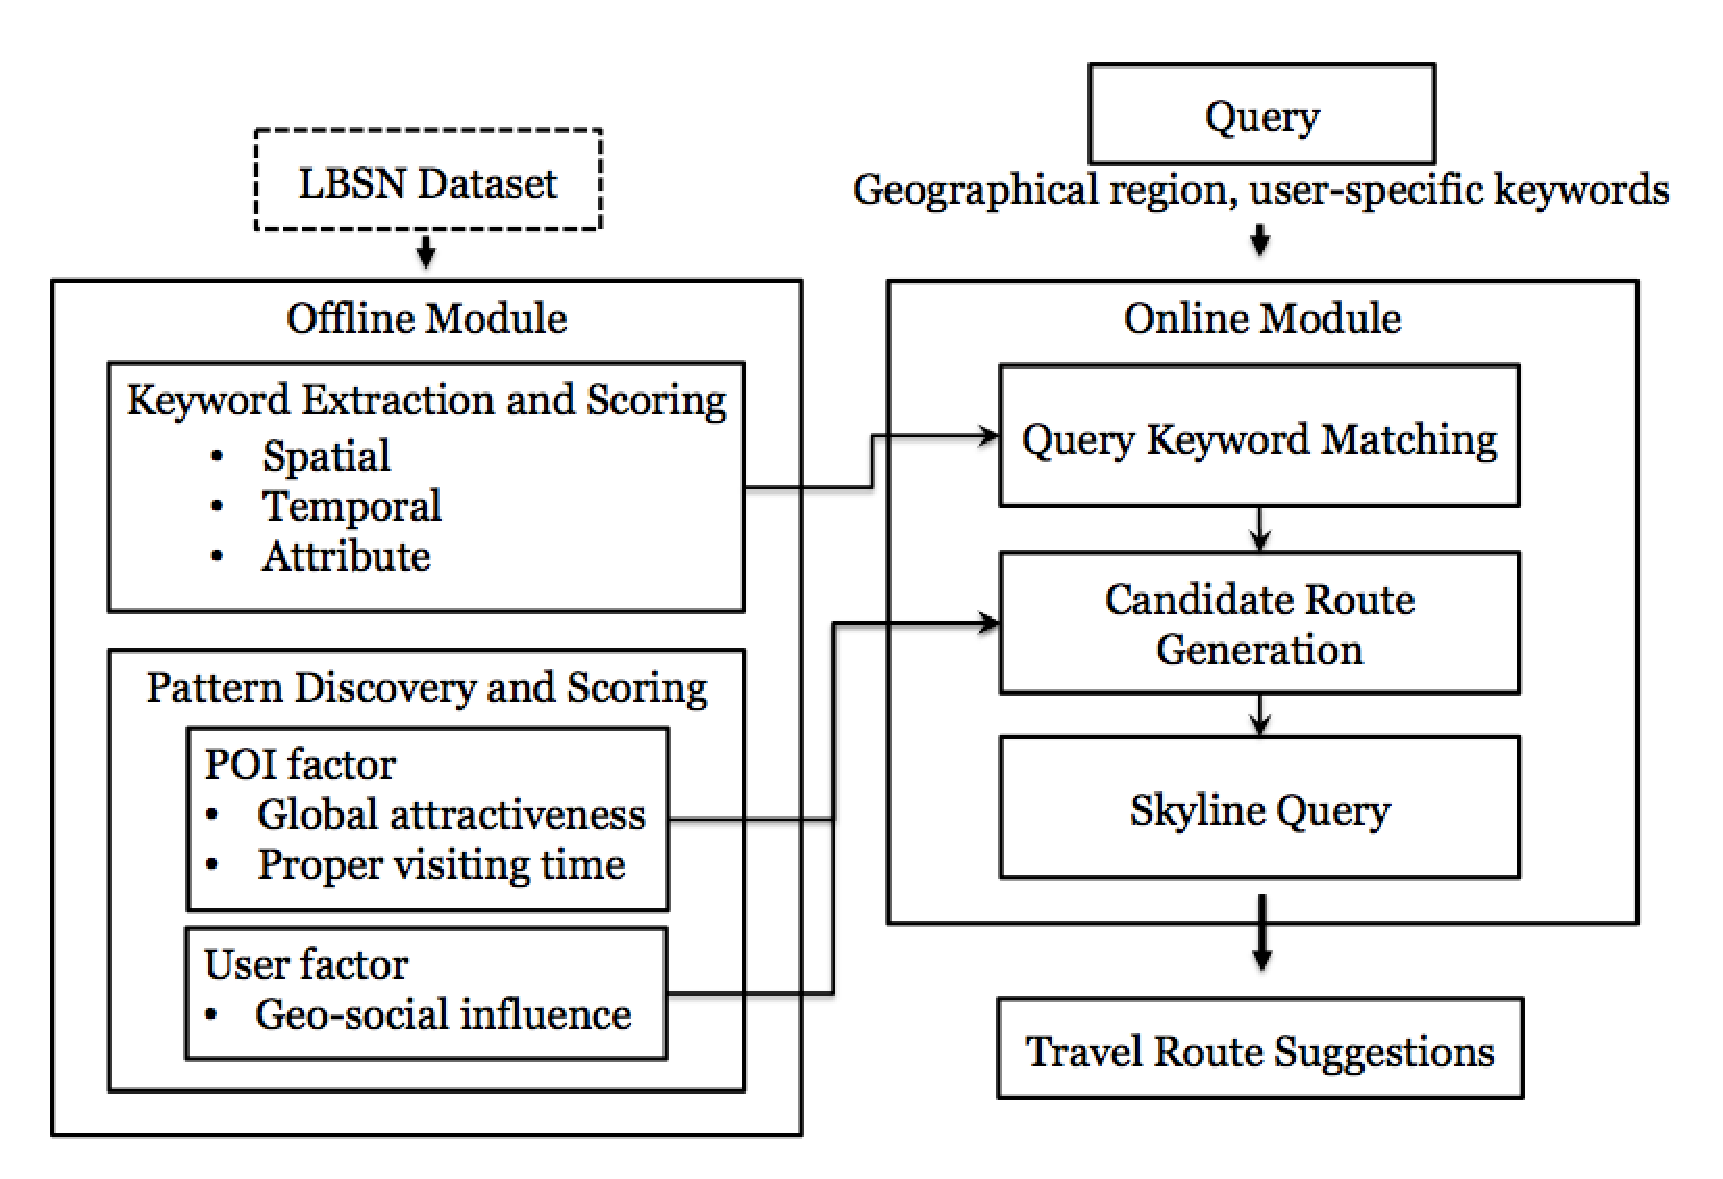
\includegraphics[width=\linewidth]{framework.eps}
\caption{The overview of the proposed \textit{Keyword-aware Skyline Travel Route} framework}
\label{fig:framework}
\end{figure} 

\textbf{Offline pattern discovery and scoring module:} Given an LBSN dataset, we first analyze the tags of each POI to determine the semantic meaning of the keywords, which are classified into (i) Geo-specific keywords, (ii) Temporal keywords and (iii) Attribute keywords according to their features. Then, we define the attractiveness scores and the proper visiting time of the POIs. For this goal, we translate the trajectories into a region transition graph, in which the vertices represent POIs and edges indicate the transition relationships among POIs. Furthermore, we determine the proper visiting time of each POI by analyzing the population distribution with timestamps, and assigning a time score for each time interval. Besides the global features that produce the same results for different people, social influence considers the geo-social networks for each user. In short, the main task of the offline module is to decide a set of POIs and derive their scores for each feature.

\textbf{Online travel routes exploration module:} In this module, we provide an interface for users to specify query ranges and preference-related keywords. With the map interface provided, users could simply input their query range as a rectangle, decide the time period to stay, and add keywords for personalized preference. Once it receives a specified range and time, the online module will retrieve those trajectories that overlap the query range and reconstruct proper travel routes in the stay time period. Then, the online module will compute a matched score of how well the trajectory is connected to the keywords. Consequently, the online module returns the most representative trajectories considering the aforementioned three scores to the users in our trajectory search Web interface. % The detailed design for the online module will be described later.
\section{Keyword Extraction and Pattern Discovery}\label{sec:offline}
% brief explain
This section describes an offline process of the scoring mechanism for keywords and POIs and pattern discovery from trajectory histories.
\subsection{Keyword Extraction} \label{subsec:KE}
In this subsection, we present how we extract the semantic meaning of the keywords and propose a matched score to describe the degree of connection between keywords and trajectories. The keyword extraction module first computes the spatial, temporal and attribute scores for every keyword $w$ in the corpus. At query time, each query keyword will be matched to the pre-computed score of matching $w$.

\subsubsection{Geo-specific keywords} 
Some tags are specific to a location, which represents its spatial nature.
To quantify the geo-specificity of a tag, an external database identifies geo-terms in the overall tag set and then the tag distribution on the map rates the identified geo-terms. Specifically, to identify name tags, we leverage an external geo-database. In Microsoft Bing services, Geocode Dataflow API (GDA) \footnote{https://msdn.microsoft.com/library/ff701733.aspx} can query large numbers of geo-terms and their representative locations. For a tag $w$, using GDA, we set $GDA(w)$ as 1 if its location is returned, and 0 otherwise. Then, using the geographic distribution of the tags, we can find place-level geo-terms like `Taipei101' in noisy geo-terms. Country-level geo-terms like `USA' and city-level geo-terms like `Seattle' are far more widely distributed on the globe than place-level geo-terms. Thus, we compute the variance $GeoVar(w)$ of the $(latitude,longitude)$ set including a tag $w$. With these features, we define a geo-specificity (\textsf{GS}) score of a tag $w$ as:
\begin{equation}
GS(w) \propto GDA(w)\cdot exp(-GeoVar(w))
\end{equation}
We consider a tag $w$ as a geo-specific keyword if $GS(w)$ is greater than a pre-defined threshold.


\subsubsection{Temporal keywords} \label{subsec:KE.temporal}% time distribution
Some tags are specific to a time interval, which represents its temporal nature. To quantify the temporal-spatiality of a tag, time distribution on a tag rates the identified temporal-terms. Using time distribution of tags, we can find tags associated with a specific time interval like `sunset'. Tags independent of time like `Taipei' are far more widely distributed in time than time-specific tags. Thus, to identify temporal-tags, we compute the variance $TimeVar(w)$ of the creation time of check-ins including a tag $w$. With these features, we define a temporal-specificity (\textsf{TS}) score of a tag $w$ as:
\begin{equation}
TS(w) \propto exp(-TimeVar(w))
\end{equation}
We consider a tag $w$ as a temporal keyword if $TS(w)$ is greater than a pre-defined threshold. Then, given a temporal keyword $w$, we generate a 2-dimensional Gaussian $\mathcal{N}_t(\mu,\sigma^2)$ that models the distribution of the occurring time of $w$ and define the associated time of $w$ as a time interval with up to two standard devations from $\mu$.


\subsubsection{Attribute keywords} \label{subsec:KE.attribute}
To find attribute keywords, we consider tags frequently associated with a POI (TF), while not with so many other POIs (IDF). To quantify the relevance between a tag and a POI, we define a ``document'' as an estimated check-in set $I_{p}$ of $p$. Using this POI-driven knowledge, our scoring conveys the POI semantic information in both TF and IDF.

Specifically, we use three types of frequencies: check-in frequency (\emph{pf}), user frequency (\emph{uf}), and POI frequency (\emph{rf}). Given a tag $w$ and a POI $p$, $pf(I_{p},w)$ is the number of check-ins that have $w$ in $I_{p}$. It is reasonable that a tag is likely to be one of the attribute tags as more check-ins of the POI have the tag. However, some users have the same tags in different check-ins causing overestimation of \emph{pf}. Similarly, $uf(I_{p},w)$ is the number of users that assign $w$ in $I_{p}$. \emph{uf} can control overestimated \emph{pf}. However, we need to filter common tags like `Travel', which also have high \emph{pf} and \emph{uf}.
Given a tag $w$ and a set $p$ of all POIs, $rf(L,w)$ is the number of POIs $p \in L$ having $w$ in $I_{p}$. Consider the $rf$ distribution on the overall tag set. The head may contain tags that would be too generic attributes for all POIs, while tags in the tail (i.e., $rf=1$) are likely not to be attribute terms. With these three types of frequencies, we define an attribute (\textsf{AT}) score of a tag $w$ as:
\begin{equation}
AT(w) \propto \max_{p \in L} \frac {pf(I_{p},w)\cdot uf(I_{p},t)}{rf(L,w)}
\end{equation}
We consider a tag $w$ as an attribute keyword if $AT(w)$ is greater than a pre-defined threshold and $rf(L,w)>1$.


\subsection{Pattern Discovery Methods}
To achieve the ``Where, When, Who'' consideration issue of user demands, the pattern discovery and scoring module defines the ranking mechanism for each POI with global attractiveness, proper visiting time and geo-social influence.

\subsubsection{Determining the attractiveness scores of POIs}
Below, we briefly introduce how to determine the attractiveness scores for POIs by mining the transition pattern.

Given a set of trajectories recorded as a series of check-in points, each check-in point represents a POI, which is denoted by $(latitude,longitude)$.

\begin{figure}[t]
 \centering
 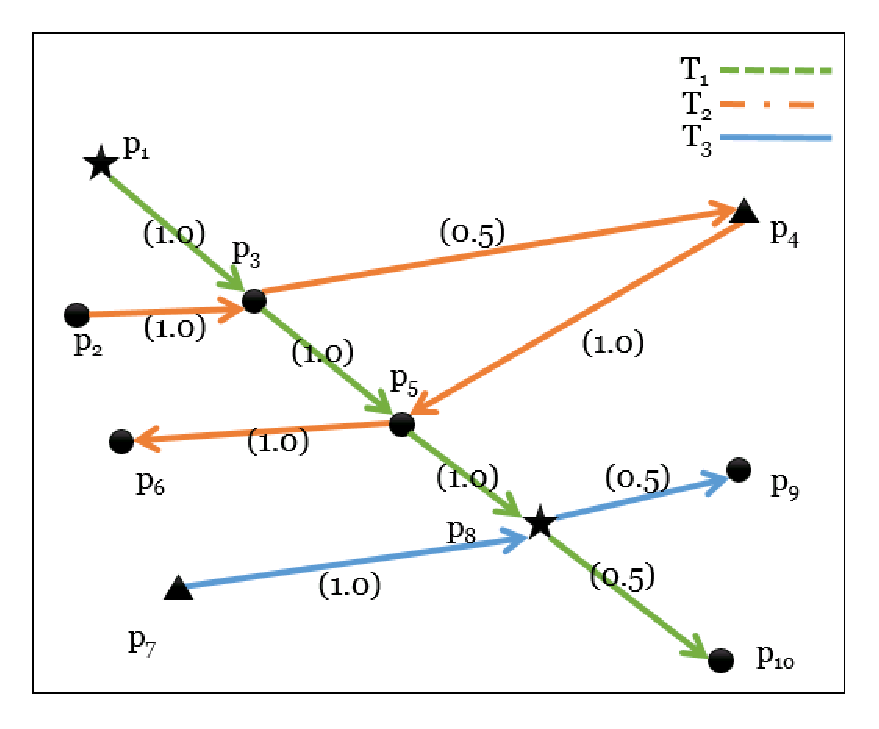
\includegraphics[width=6cm]{RWmodel_TraSearch.eps}
 \caption{An example of a region transition graph}
 \label{fig:RWmodel_TraSearch}
 \end{figure}

To measure the attractiveness of POIs, we intend to explore the sequential relationships hidden in the trajectory records. A region transition graph is built based on the transition probabilities to derive the traversal relationship. The example in Figure~\ref{fig:running_example} can be revised to a region transition graph shown as Figure \ref{fig:RWmodel_TraSearch}. The edges indicate the transition relationships among POIs. The weight of each edge is derived by aggregating the transition relationship from a set of trajectories. With the region transition graph, we borrow the concept in PATS \cite{PATS} to adopt the Markov model to assign an attractiveness score to each POI and denote the attractiveness score of POI $p_{i}$ represented as $AS(p_{i}$). According to PATS~\cite{PATS}, the attractiveness of a trajectory can be inferred by a sequence of POIs and the concept of random walks. % Based on this intuition, we developed a travel trajectory recommendation system for retrieving some interesting routes which fulfill two requirements: (i) travel routes should contain all those query points specified (ii) travel routes should within the spatial range $Q$.


\subsubsection{Proper visiting time decision} \label{sec:offline.2}
As claimed in~\cite{hsieh2012exploiting}\cite{hsieh2014mining}, the pleasure of visiting the POIs along a route is closely related to the arrival time. Some places have a wider range of visiting time period while others are constrained to certain particular time slots. For example, most people do not go to night markets in the morning, but rather arrive in the evening after the market opens. Thus, we extract time information from the timestamp of check-ins and mine the proper visiting time period of each POI. As shown in Figure \ref{fig:time_distribute}, each POI has a different time distribution curve. For example, the distribution of Shihlin Night Market in Figure \ref{fig:night} shows that most people have check-ins during the evening and we can infer that the proper visiting time of Shihlin Night Market is about 17:00 to 23:00. Another example in Figure~\ref{fig:day} shows that most people visit Shilin Presidential Residence during the daytime so the proper visiting time may be 7:00 to 17:00. When the distribution curve approaches a horizontal line, it indicates that the POI is suitable to be visited at any time. On the contrary, when the distribution curve has a peak segment, it indicates that the POI may be popular at a special time and proper to visit at that time. The same concept can be used in the case of seasons, weekends and weekdays.

Here we separate one day into 24 time intervals. We first define the probability of a POI $p$ be visited at time $t$ as ${N(p,t)}/N_{total}(p)$, where ${N(p,t)}$ is the number of people who have check-ins in $p$ at time $t$, and $N_{total}(p)$ is the total number of people who visit $p$. Due to the concern of data sparsity, we apply the 2-dimensional Gaussian $\mathcal{N}_t(\mu,\sigma^2)$ to fit the distribution of visiting time, which is similar to the idea of the temporal score in Section~\ref{subsec:KE.temporal}.
\begin{equation}
P(p,t)=\frac {1}{\sqrt{2\pi}\sigma} exp\left[ -\frac { { \left( x-\mu  \right)  }^{ 2 } }{ 2{ \sigma }^{ 2 } }  \right] 
\end{equation}

After defining the visiting probability, we define the visiting time score $VS(p,t)$ for POI $p$ at time $t$ between 0 and 1 as:
\begin{equation}
VS(p,t)=\frac{P(p,t)}{max_{t\in{0{\rightarrow}23}}(P(p),t)}
\end{equation}
where $max_{t\in{0{\rightarrow}23}}(P(p),t)$ is the maximum probability of visiting $p$ in one day.

\begin{figure}[t]
\centerline{
\mbox{
    \subfigure[Shihlin Night Market]{
        \label{fig:night}
        \includegraphics[width=0.55\linewidth]{Shihlin_night_market.eps}
    }
    \subfigure[Shihlin Residence]{
        \label{fig:day}
        \includegraphics[width=0.55\linewidth]{Shihlin_Residence.eps}
    }
}}
\caption{The distributions of the visiting probability at each time unit (hour) for (a)Shihlin Night Market, and (b)Shilin Presidential Residence from check-in records.}
\label{fig:time_distribute}
\end{figure}

Now we give an example to illustrate how to compute $VS$. Given a visiting time Gaussian distribution of $p$ in Figure \ref{fig:time_ex}, the maximum visiting time probability of $p$, i.e., $max(P(p))$ is 0.08 at the 19:00 time interval, the probability of the 10:00 interval is 0.04, and $VS(p,10)=0.04/0.08=0.5$.

% need to revised! %%%%%%%%%%%%%%%
\begin{figure}[t]
\centering
\includegraphics[width=0.8\linewidth]{time_ex.eps}
\caption{An example of visiting time scoring. Two-dimensional Gaussian distribution is adopted to deal with inconsistent data due to data sparsity.}
\label{fig:time_ex} % 一定要在 caption 之後
\end{figure}

\subsubsection{Geographical social influence}
Another important feature in POI recommendation is the social influence of each user. The closer the relationship between two users, the more reliable the recommendation is. We focus on the condition that if user $u_i$ is socially influenced by user $u_j$, $u_i$ would visit a POI because of the recommendation from $u_j$. We can observe a relation that $u_i$ checks in at the same POI $p$ after $u_j$ shared her/his check-in. \cite{ytwen2014} proposed a Social Influence Recommender (SIR) framework to explore the influential users in an LBSN. The main issue is to capture the interaction among the social network, physical locations and time effect by defining the geo-social following relation among users. Then a diffusion model is utilized to stimulate the influence spreading process. The example in Figure~\ref{fig:running_example} can also be revised to Figure \ref{fig:sir_example} to measure the geo-social influence among users.

\begin{figure}[h]
\begin{center}
\begin{tabular}{ccc}

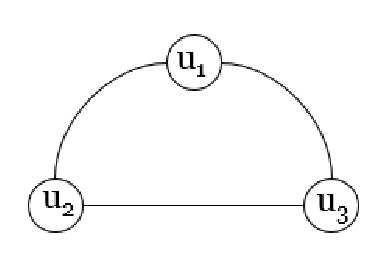
\includegraphics[scale=0.5]{sir_1.eps} &
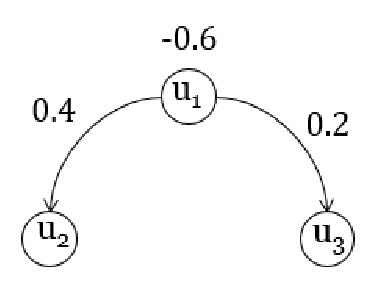
\includegraphics[scale=0.5]{sir_2.eps}
\\
(a) Social graph & (b) Following graph
\\
\multicolumn{2}{c}{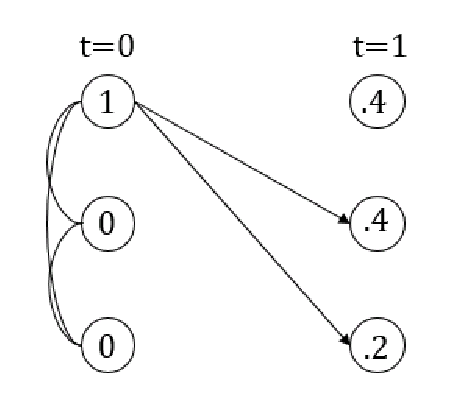
\includegraphics[scale=0.5]{sir_3.eps}}
\\
\multicolumn{2}{c}{(c) Influence propagation from t = 0 to t = 1}

\end{tabular}
\end{center}
\vspace{-3mm}
\caption{An example of influence propagation among three users.}
\label{fig:sir_example}
\end{figure}

The social influence can propagate among the users within the \textit{following graph}. Formally, the amount of influence transited from ${u_i}$ to ${u_j}$ is defined as ${f_{ij}=\frac{p(u_i,u_j)}{n(u_i)}}$. ${p(u_i, u_j)}$ denotes the probability of geo-social following relationships of ${u_i}$ to ${u_j}$, and ${n_i}$ denotes the total number of locations ${u_i}$ has visited. \cite{ytwen2014} assumes that user ${u_i \in V}$ is only influenced by her/himself initially and the influence will be propagated to others in the  \textit{following graph} afterwards. During the propagation process, users receive stimulation from their neighbors. Finally, vector ${s(t)}$ denotes the proportion of the social influence score on users in $V$ at time $t$, the change at ${u_i}$ between time ${t+\Delta t}$ is defined by the following equation using the diffusion model:
%since the first $\textit{follow}(C(u_i,l,t),u_j,\delta)$ happened

\begin{equation}\label{eq:diffusion}
\frac{s(t+\Delta t)-s(t)}{\Delta t}=\alpha Inf s(t)
\end{equation}

where ${\alpha}$ is the propagation coefficient and $Inf$ is a matrix which defines the one-hop information diffusion process. 

\section{Travel route exploration} % reconstruction -> pruning -> skyline
In this section, we present the algorithm of trajectory reconstruction and how to apply Skyline query for our online recommendation system. Furthermore, we propose an approximate algorithm to speed up the real-time Skyline query. The \textit{Travel Route Exploration} procedure is presented as Algorithm~\ref{algo:TR}.

\begin{algorithm}[h]
\label{algo:TR}
  \caption{Travel routes exploration}
  \small
  \Indm
  \KwIn{Specific user $u$,
    query range $Q$,
    a set of keywords $K$ and threshold $\epsilon$;}
  \KwOut{Keyword-aware travel routes with diversity in goodness domains \textit{KST}.}
  \Indp
  Initialize priority queues \textit{CR,KST};\\
  Scan the database once to find all route histories covered by region $Q$;\\
  \tcc{Fetch POI scores and check keyword matching}
  \ForEach{route $r$ found} {
    \textit{r.kmatch} $\leftarrow$ 0;\\
    \ForEach{POI $p$ $\in$ $r$} {   
      \textit{r.kmatch} $\leftarrow$ \textit{r.kmatch} + KM(p,k);\\
    }
    \If{r.kmatch $>$ 0}{
      Push $r$ into \textit{CR};\\
    }
  }
  \tcc{Candidate route generation, see Algorithm 2}
  Append Reconstruct(\textit{CR}) to \textit{CR};\\
  \tcc{Skyline search}
  \ForEach{route $r$ $\in$ \textit{CR}} {
    %\If{Keyword-Match($r$,$K$,$\epsilon$)} {
    \ForEach{candidate route $r_c$ $\in$ $KST$} {
      \If{ $r_c$\textit{.score} dominates \textit{r.score} } {
        $r$ is discarded as not part of the skyline;
      }
      \If{ \textit{r.score} dominates $r_c$\textit{.score} } {
        Pop $r_c$ from \textit{KST};
      }
      Push $r$ into \textit{KST};
    }
    %}
  }
  \KwRet{\textit{KST}.}
\end{algorithm} 

 % \subsection{Query Keyword Matching} \label{subsec:KM}
 \subsection{Query Keyword Matching} \label{subsec:KM}
To process the user queries, we first describe how to match query keywords with the characteristic scores assigned to tags. The user-specific keywords in the query reflect the individual's preferences regarding the trip, i.e., the user tends to choose a travel route that contains POIs closely related to the semantic meanings. In the offline model, we have built a tag corpus for POIs with characteristic scores and metadata. Also, relevant tags for each POI are weighted in the TFIDF manner. Given a keyword set $K$ and arbitray POI $p$ at query time, we define a keyword matching measure \textbf{KM} with the pre-computed information:
\vspace{-1.5mm}
\begin{equation}
KM(p,K) = \sum_{k \in K}{tfidf(k,p) \cdot (GS(k)+TS(k)+AT(k))}
\end{equation}
where \textit{tf} is the frequency of tag $k$ in a POI and \textit{idf} is the number of POIs with the tag $k$.

For example, consider that given the keyword set $K$ = [``night'' ``ximending''], we then find the temporal score of ``night''= 0.9 and the geo-specific score = 0.001; the temporal score of ``ximending'' = 0.5 and the geo-specific score = 0.95. On the other hand, in a POI ``red house'', the TFIDF score of night = 0.3 and the TFIDF score of ximending = 0.8. These scores of keyword set $K$ can be aggregated for POI ``red house'' as score (0.3 $\times$ (0.9 + 0.001) ) + (0.8 $\times$ (0.5 + 0.95) ). For the route with multiple POIs, the score of each POI as computed above will be summed up. The higher the score, the more related the route is with the keyword. We filter out the routes with zero score, which means that those routes are not related to the user's preference. 

\subsection{Candidate Route Generation} \label{subsec:online.2}% dynamic 
We have proposed the method for matching raw texts to POI features in each travel route candidate to fulfill the requirement that recommended travel routes should connect to all or partial user-specific keywords. Notice that the trajectories found in the previous section are limited to the existing trajectories. However, the existing trajectories sometimes may not include all the query criteria, and may have bad connections to the query keywords. Thus, we propose the \textit{Candidate Route Generation} algorithm to combine different trajectories to fit the query requirement.  

The new candidate routes are constructed by combining the subsequences of trajectories. Here we introduce the pre-processing method first. We then utilize the pre-processing results to accelerate the proposed route reconstruction algorithm. Last, we design a Depth-first search-based procedure to generate possible routes.

 \textbf{Pre-processing:} After the \textit{Query Keyword Matching} check, all the input routes must have at least one user-specific keyword. With the information that a trajectory $T_{i}$ consists a sequence of POIs, \{$p_{1},p_{2},...p_{n}$\}. Then we use the data structure (head,tail) to reinterpret the trajectory for one-step transition, i.e., \{$p_{1}\rightarrow p_{2},p_{2}\rightarrow p_{3},...,p_{n-1}\rightarrow p_{n}$\}. Two dictionaried lists $headSet$ and $tailSet$ are used to record the head and tail records respectively.
 
 \textbf{Combined points should be ordered by time:} Obviously, it is intuitive to combine ($p_{i},p_{j}$) and ($p_{k},p_{l}$) if $p_{j}$ and $p_{k}$ are the same location. Besides considering spatial distance, we also need to consider the visiting time order among combined points. Since \textit{tail.time} must be larger than \textit{head.time}, \textit{$p_k$.time} should be larger than \textit{$p_i$.time} in order to replace $p_j$ by $p_k$.
 
 \textbf{DFS-based route enumeration:} In order to generate all possible routes from original trajectories, we reconstruct new trajectories by linking the (head,tail) subsequences using combined point. This would be a depth-first search-based procedure. We consider all the POIs in the headSet as source, and explore as far as possible along each link before backtracking. Furthermore, it is relatively straightforward to consider the time-period query in the process of DFS. In Algorithm 2, we only need to add a more strict time-query limitation to line 7, e.g., the size of $S$ should not exceed a \textit{the number of POIs in a route} threshold.


For example, the three existing travel routes $T_{1}$, $T_{2}$ and $T_{3}$ from Figure~\ref{fig:running_example} can be reinterpret into (head,tail) pairs, as shown in Table II. Then we have the $headSet$ \{$p_1$,$p_2$,$p_3$,$p_4$,$p_5$,$p_7$,$p_8$\}. Start from $p_1$, \{$p_1$ (10:00) $\rightarrow$ $p_3$ (12:00)\} is found first. $p_3$ is the combined point to \{$p_3$ (12:30) $\rightarrow$ $p_4$ (17:00)\} since the visiting time order is correct. Finally, a candidate route $T'_4$ is generated as \{$p_{1}$ (10:00) $\rightarrow$ $p_{3}$ (12:30) $\rightarrow$ $p_{4}$ (17:00) $\rightarrow$ $p_{5}$ (19:00) $\rightarrow$ $p_{6}$ (19:30)\}. Table III shows the result of candidate routes: $T_1$ - $T_3$ are original routes and $T'_4$ - $T'_6$ are three of the reconstructed routes. 

\begin{algorithm}[t]
\label{algo:CRG}
\caption{Candidate Route Generation}
\small
\Indm
\KwIn{Route set $R$;}
\KwOut{Candidate route set $CR$.}
\Indp
Initialize a stack $S$, priority queue $CR$;\\
Split $r$ $\in$ $R$ into (head,tail) subsequences;\\
Reconstruct(headSet).\\ 
Procedure Reconstruct(Set):\\
  \ForEach{(head,tail) $\in$ Set}{
    endFlag = False;\\
    \If{S is empty or tail.time $>$ S.pop().time}{
      Push head in $S$;\\
      Push tail in $S$;\\
    }
    \Else{
      Push head in $S$;\\
      endFlag = True;\\
    }
    \If{endFlag is False}{
      Reconstruct(tailSet)
    }
    Add $S$ in $CR$;\\
  } 
Procedure End\\
\end{algorithm}

\begin{table}[h]
 \centering
 \caption{Raw trajectory dataset.}
 \begin{footnotesize}
 \begin{tabular}{|l|l|l|} \cline{1-3}
Tid & \multicolumn{2}{c|}{(head,tail) subsequence} \\ \hline
\multirow{2}{*}{$T_{1}$} & $p_{1}$ (10:00) $\rightarrow$ $p_{3}$ (12:00) & $p_{3}$ (12:00) $\rightarrow$ $p_{5}$ (15:30) \\ \cline{2-3}
                         & $p_{5}$ (15:30) $\rightarrow$ $p_{8}$ (17:30) & $p_{8}$ (17:30) $\rightarrow$ $p_{10}$(19:00) \\ \cline{1-3}
\multirow{2}{*}{$T_{2}$} & $p_{2}$ (10:30) $\rightarrow$ $p_{3}$ (12:30) & $p_{3}$ (12:30) $\rightarrow$ $p_{4}$ (17:00) \\ \cline{2-3}
                         & $p_{4}$ (17:00) $\rightarrow$ $p_{5}$ (19:00) & $p_{5}$ (19:00) $\rightarrow$ $p_{6}$ (19:30) \\ \cline{1-3}
$T_{3}$                  & $p_{7}$ (18:30) $\rightarrow$ $p_{8}$ (19:30) & $p_{8}$ (19:30) $\rightarrow$ $p_{9}$ (20:00) \\ \hline
\end{tabular}
 \end{footnotesize}
 \label{Tab:raw_trj}
 \end{table}

\vspace{-2mm}

 \begin{table}[h]
 \centering
 \caption{Subset of Candidate Routes.}
 \begin{footnotesize}
 \begin{tabular}{|c|l|} \hline
 Tid & POI sequence\\ \hline
 $T_{1}$ & $p_{1}$ (10:00) $\rightarrow$ $p_{3}$ (12:00) $\rightarrow$ $p_{5}$ (15:30) $\rightarrow$ $p_{8}$ (17:30) $\rightarrow$ $p_{10}$(19:00)\\ \hline
 $T_{2}$ & $p_{2}$ (10:30) $\rightarrow$ $p_{3}$ (12:30) $\rightarrow$ $p_{4}$ (17:00) $\rightarrow$ $p_{5}$ (19:00) $\rightarrow$ $p_{6}$ (19:30)\\ \hline
 $T_{3}$ & $p_{7}$ (18:30) $\rightarrow$ $p_{8}$ (19:30) $\rightarrow$ $p_{9}$ (20:00) \\ \hline
 $T'_{4}$ & $p_{1}$ (10:00) $\rightarrow$ $p_{3}$ (12:30) $\rightarrow$ $p_{4}$ (17:00) $\rightarrow$ $p_{5}$ (19:00) $\rightarrow$ $p_{6}$ (19:30)\\ \hline
 $T'_{5}$ & $p_{1}$ (10:00) $\rightarrow$ $p_{3}$ (12:00) $\rightarrow$ $p_{5}$ (19:00) $\rightarrow$ $p_{6}$ (19:30)\\ \hline
 $T'_{6}$ & $p_{1}$ (10:00) $\rightarrow$ $p_{3}$ (12:00) $\rightarrow$ $p_{5}$ (15:30) $\rightarrow$ $p_{8}$ (19:30) $\rightarrow$ $p_{9}$ (20:00)\\ \hline
 \end{tabular}
 \end{footnotesize}
 \label{Tab:re_trj}
 \end{table}

%Notice that a reconstructed trajectory is combined from the  fragments of different trajectories, the different trajectories may visit the same POI in the different time. Thus, in order to decide the visiting time of POI for reconstructed trajectory, we align the visiting time of the POI by making the Combined Points of two trajectory visited in the same time. We choose the timeline of one trajectory with more contribution to the visiting time scores of query points as base timeline, and align the visiting time of another trajectory to this timeline. For example, assume A and D are query points in figure \ref{fig:TimeAlign},we get a reconstructed trajectory $Trj_{ij}$ by combining $Trj_{i}$ and $Trj_{j}$ using B as Combined Points. If the timeline of $Trj_{j}$ has more contribution to the visiting time score of query points, we align the visiting time of B in $Trj_{i}$ from 10:10 to 8:20, and  also set the visiting time of the POI before B for one hour and fifty minutes earlier. The result of reconstructed trajectory will be 7:30 A$\rightarrow$8:20 B$\rightarrow$12:10 D$\rightarrow$14:40 E. Finally, we set the matched score as summation of the visiting time score for Skyline Travel Route.

\subsection{Skyline Travel Routes Search}
 Given a data set $D$, a Skyline is a subset of data which stands out among others and is of special interest to us in $D$. More formally, a Skyline is a subset of data in D which is not dominated by any others. Let $a$ and $b$ be data points in D, $a$ dominates $b$ if $a$ is as good as or better than $b$ in all dimensions and better in at least one dimension. Instead of using a traditional recommendation system considering a fixed weighting for a set of criteria and returning the top $K$ trajectories with the highest score, Skyline query considers all possible weighting criteria that might offer an optimal result. 

 Unlike the top-$K$ system where users are required to specify weighting for a set of criteria and retrieval size $K$, Skyline does not need to make such a difficult decision. To illustrate, we have given an example of Skyline in the introduction and described the three scoring criteria in previous sections. Now we give the definition of the travel route Skyline as follows:

\begin{defi}(Skyline travel route):
Given a trajectory set, we have already retrieved the scores of attractiveness, time, and geographical social influence scores in the previous sections. The results of the Skyline travel route are not dominated by any other trajectory. Consider the three dimensions previously mentioned, i.e., attractiveness, time, and geographical social influence score; trajectory $T_{i}$ dominates trajectory $T_{j}$ if and only if the score of $T_{i}$ in any dimension is not less than the corresponding score of $T_{j}$, where $i$ is not equal to $j$.
\end{defi}

In other words, the user need not specify the weight between every criteria on first because travel route Skyline returns all the possible optimal results w.r.t. arbitrary weight. In our system, the user can choose the travel route considering the different weight in three dimensions: (i) how attractive this trajectory is, (ii) the proper visiting time of each POI in the travel sequence, and (iii) the social influence of the users who have visited the POI. Each trajectory is regarded as a three-dimensional data point and each dimension corresponds to one score. After computing the trajectory scores, we return the Skyline travel routes as the recommended travel routes.

% Also, there exist some efficient algorithms for calculating Skyline queries in the database. In \cite{BBS}, the authors propose an efficient IO optimal method, called BBS. % R-tree index
\vspace{-2mm}

\subsection{Greedy Pruning}
Recall Section~\ref{subsec:online.2}, a brute-force approach to generate the candidate routes is to enumerate all subsequences. The time complexity of candidate route generation is $\mathcal{O}(n^l)$, where $n$ is the number of original routes and $l$ is the average length of the routes. Also, the amount of reconstructed routes is $\mathcal{O}(n^l)$ because the routes are generated during the traversal. Since we only require the Skyline results, the redundant time cost of computing the scores and searching for low-ranked routes is computationally prohibitive. %Afterwards, we design a greedy pruning algorithm to reduce the size of POI elements in the routes.

As discussed in Section~\ref{sec:offline}, there are three dimensions to be considered in a Skyline search. Generally, POIs with higher scores in each dimension have higher probability not to be dominated. We leverage a greedy pruning method to reduce the number of candidate routes. The idea is that we only use the top-$N$\% ranked POIs to construct routes. We define the greedy score of POI element $p$ as 
\begin{equation}
GPscore(p) = p.patscore+p.timescore+p.socialscore
\end{equation}

In particular, the greedy pruning should be applied before the candidate route generation, and then use the pruned results to reconstruct candidate routes. % Note that the score of geographical social influence is not considered here because we. 

\begin{algorithm}[h] 
  \caption{Greedy Pruning Algorithm}
  \label{algo:GP}
  \small
  \Indm
  \KwIn{Route set $R$,
  pruning threshold $N$\%;}
  \KwOut{Route set after greedy pruning \textit{GPR}.}
  \Indp
  \ForEach{route $r$ found} {
    \textit{r.gpscore} $\leftarrow$ 0;\\
    \ForEach{POI $p$ $\in$ $r$} {   
      \textit{r.gpscore} $\leftarrow$ \textit{r.gpscore} + GPscore(p);\\
    }
  }
  Sort $R$ with $r.gpscore$;\\
  \textit{GPR} $\leftarrow$ top-$N$\% of $R$;\\
  \KwRet{\textit{GPR}.}
\end{algorithm}

% complexity
 The sorting takes $\mathcal{O}(n\log{}n)$ time and then the procedure of candidate route generation can be reduced to $\mathcal{O}(n^{N\%\times l})$. Moreover, the time cost on Skyline search decreases exponentially as the number of candidate routes decreases. So we get the approximate results efficiently.

\subsection{System Implementation} \label{sec:implementation}
We implemented the system on an x86\_64 Linux server with 16 cores and 8 GB memory. All the scores mentioned in Section~\ref{sec:offline} are computed offline and stored in a PostgreSQL 9.3 database with GIS extension. %To be efficient with massive computations, we optimize the implementation by using MapReduce framework to parallelize the independent computations.

Assume the number of routes in the dataset is $N$, and the average length of the routes is $l$. The time complexity of our \textit{Travel Route Exploration} algorithm depends on three parts: (i) scan the whole database to find the routes in the query range, (ii) generate candidate routes and (iii) calculate feature scores and run Skyline search on all generated candidate routes. First, the search for (i) takes $\mathcal{O}(N)$ and gets even faster since the R-tree based GIS index filters out non-candidate routes efficiently. For step (ii), we have proposed a approximate mechanism to reduce the computations. And for each candidate route, step (iii) computes the scores and compares the domination to other routes. The complexity is $\mathcal{O}(N^2\times l)$. In the case of extensive routes returned from a large-scale query region, it leads to excessive computational time and is not applicable for an interactive online system. We optimize the implementation by parallelizing score comparison in step (iii), which involves independent computations of each route. See Section~\ref{sec:exp_run_time} for the optimized run time results.

% \begin{figure}[h]
% \centering
% 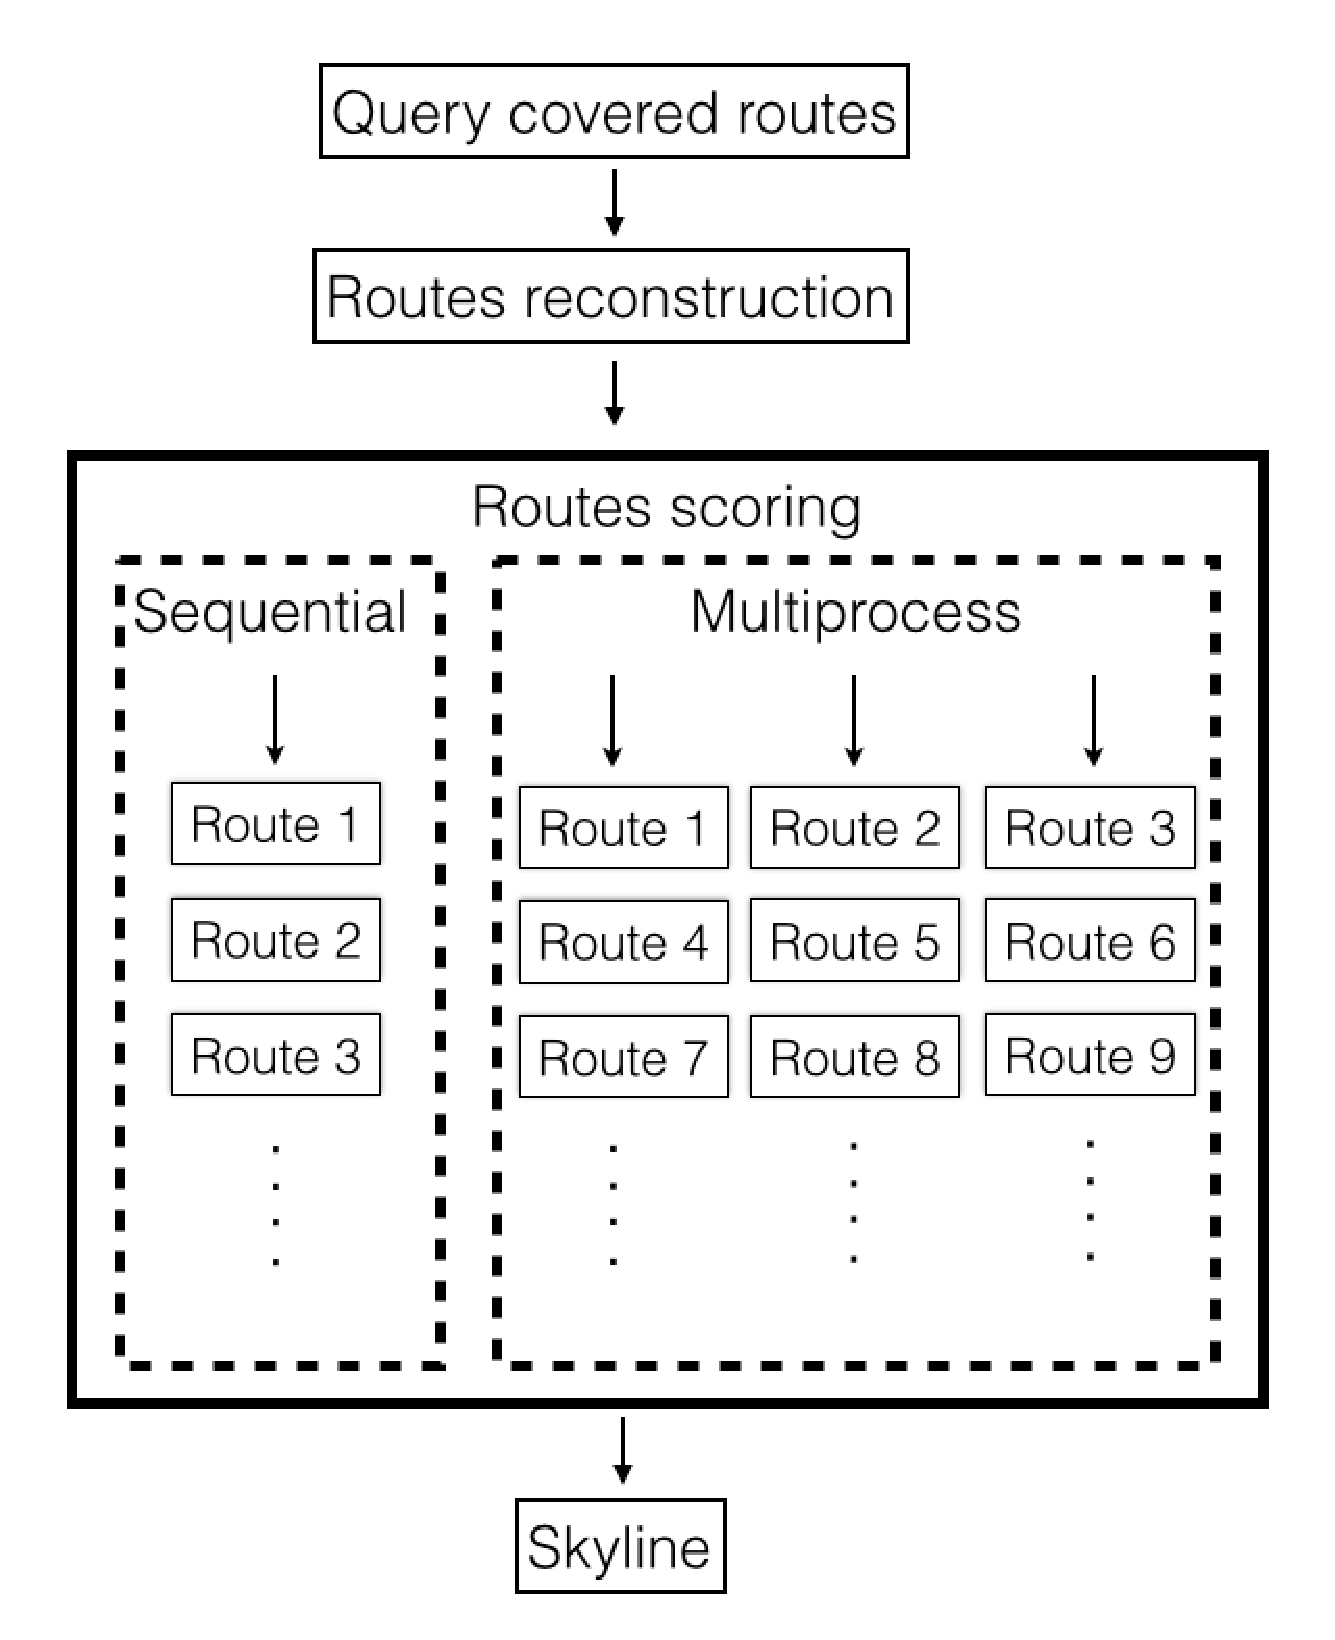
\includegraphics[width=4.5cm]{implementation.eps}
% \caption{Muiti-processing in system implementation.}
% \label{fig:implementaion}
% \end{figure}

% Data structure

 \section{Experiments}
 In this section, we empirically evaluate the effectiveness and efficiency of the proposed algorithms. First, we describe the baseline approaches and evaluation methodology of the experiments. We use two real-world LBSN datasets shown in Table IV. The \textit{FB} dataset is collected by Facebook API\footnote{Facebook Developers. https://developers.facebook.com/}. We have taken 96 volunteers' Facebook accounts as user seeds (most of the users live in Taiwan) and crawled all their and their friends' location records (i.e., check-ins and geo-tagged photos) over the period of Jan. 2012 - Dec. 2014. \textit{CA} is another Foursquare dataset with an undirected friendship network from~\cite{gao2012exploring}. All the experiments are conducted on an x86\_64 Linux server with 16 cores and 8 GB memory. %The \textit{GWL} dataset\footnote{Stanford Network Analysis Project (SNAP). http://snap.stanford.edu/data/loc-gowalla.html} and \textit{FS} are two check-in datasets with an undirected friendship network. Note that \textit{GWL} and \textit{FS} are larger datasets but lack with the information of POI categories.

\begin{table}[h]
\begin{center}
\caption{Details of the LBSNs}
\footnotesize{
\begin{tabular}{|l|c|c|c|}
  \hline
   & Property & \multicolumn{2}{|c|}{Network} \\ \cline{3-4}
   & & \textbf{FB} & \textbf{CA}\\
  \hline
   \#records & check-in & 869,317 & 483,813\\
  \hline
   \#nodes & user & 29,512 & 4,163\\
   & POI & 225,077 & 121,142\\
  \hline
   \#edge & friend & 39,513 & 32,512\\
  \hline
\end{tabular}}\\
\end{center}
\label{table:data.des}
\vspace{-1.3mm}
\end{table}

To gain insights into the datasets, we plot both the number of check-ins and routes of each user of our datasets. As shown in Figure~\ref{fig:exp_obs}, the number of check-ins and routes for each user is highly skewed in both datasets. Moreover, all distributions have long tails. In particular, the top 10\% ranked users in all datasets have nearly 60\% of total check-ins and routes. This indicates that most of the users are quite inactive. The data sparsity issue may cause considerable bias on the result of inactive users. So we chose the top 10\% of users, who were ranked by the travel route histories they have, as active users for testing. 
% 和沒有sample有何差別

\begin{figure}[h]
\centering
\mbox{
    \subfigure[Check-in distribution of \textit{CA} dataset]{
        \label{fig:exp_obs1}
        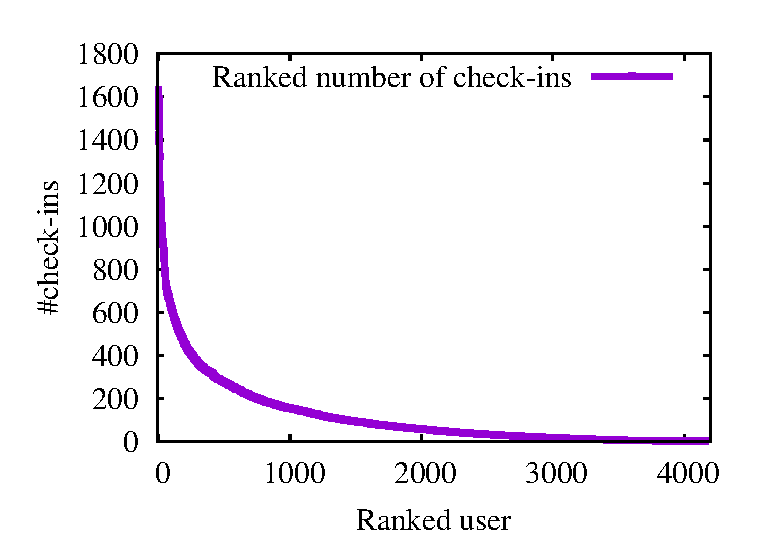
\includegraphics[width=0.48\linewidth]{obs_checkin_ca.eps}
    }
    \subfigure[Check-in distribution of \textit{FB} dataset]{
        \label{fig:exp_obs2}
        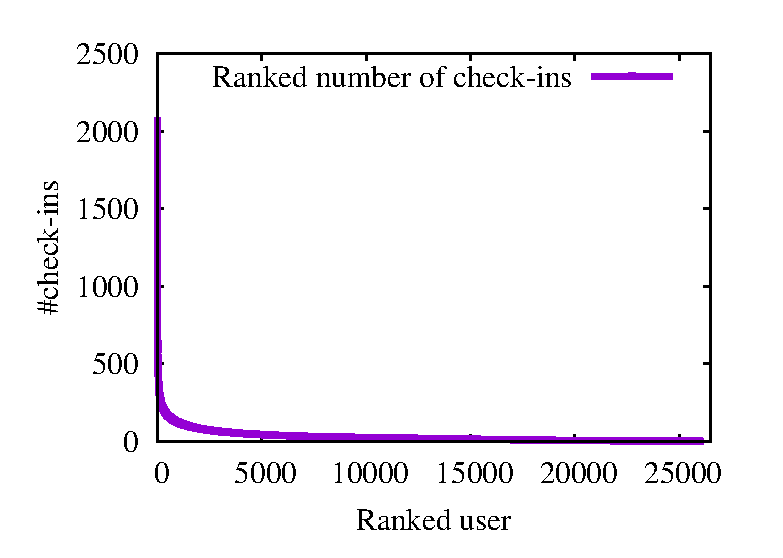
\includegraphics[width=0.48\linewidth]{obs_checkin_fb.eps}
    }
}
\mbox{
    \subfigure[Route distribution of \textit{CA} dataset]{
        \label{fig:exp_obs3}
        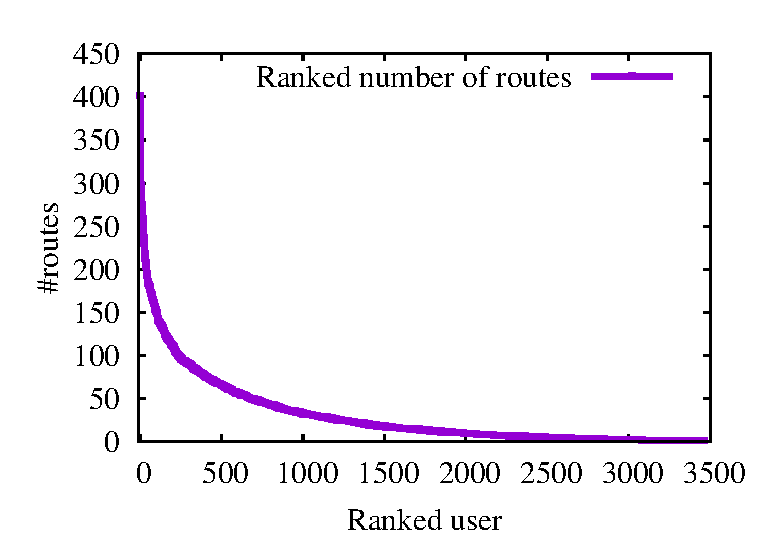
\includegraphics[width=0.48\linewidth]{obs_route_ca.eps}
    }
    \subfigure[Route distribution of \textit{FB} dataset]{
        \label{fig:exp_obs4}
        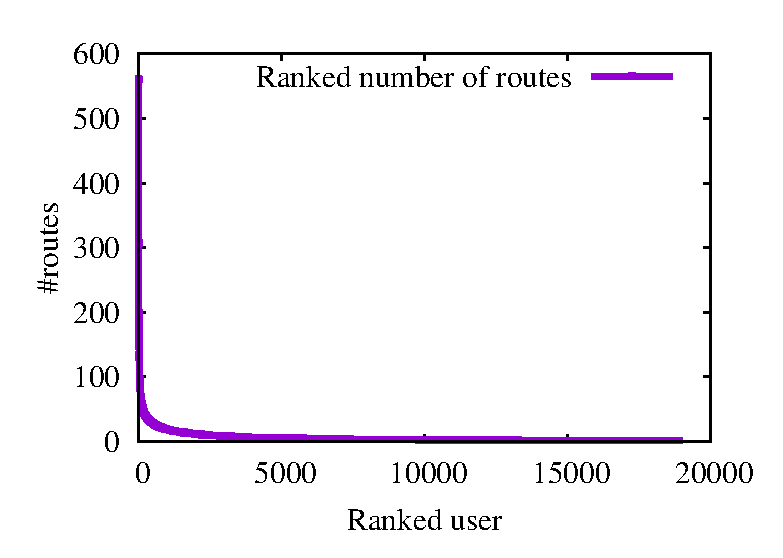
\includegraphics[width=0.48\linewidth]{obs_route_fb.eps}
    }
}
\caption{The number of check-ins and the number of routes for all uses in \textit{CA} and \textit{FB} dataset, respectively. The distribution shows a long tail extending in the negative direction.}
\label{fig:exp_obs}
\end{figure}

% \subsection{Keyword matching accuracy}
\subsection{Keyword matching accuracy} \label{sec:exp.keyword}

In this subsection, we evaluate the quality of the extracted keywords. Since our check-in datasets do not have sufficient text descriptions, i.e., tags, we collected an additional photo dataset consisting of 165,057 photos with 958,441 tags in the same local area. For that, the tags are regarded as input keyword. We ranked the tags by using scores in Section III-A and measured precision@$K$. Table V shows the precision of deciding  the Geo-specific, Temporal, and Attribute keywords.\footnote{For attribute extraction, we adopt~\cite{lee2013attribute} extracting probable attributes of all possible concepts. We can adopt 10 concepts aligned with POI categories, and Table VI illustrates attributes of `Food' concept for restaurant POIs.} We can see that the precision is reasonably high and does not decrease much as $K$ increases. Table VI shows the results for keyword extraction. Note that the keywords in italics are the Chinese keywords returned, which we translate for presentation. In the geo-specific dimension, 10 keywords referring to certain places are highly ranked. For example, a keyword `Longshan' represents `Longshan Temple'. In the temporal dimension, there is no doubt that keywords such as `Sunset', `Sunrise', `Lunch' and `Night' are specific to a certain time interval. `Dadaocheng' is ranked high as it is a place famous for its sunset. Also, `Butterfly' and `Fireworks' are strongly associated with day time and night time respectively. In the attribute dimension, keywords relevant to restaurant POIs are highly ranked.

\begin{table}[h]\scriptsize
\begin{center}
\caption{Precision of keyword extraction}
\vspace{1mm}
{\scriptsize\begin{tabular}{ | c | c | c | c |}
    \hline
     & P@10 & P@20 & P@40 \\ \hline\hline
    Geo-specific keyword &  1.000&  1.000& 0.975 \\ \hline
    Temporal keyword &  0.900&  0.700& 0.720 \\ \hline
    Attribute keyword & 1.000&  0.850& 0.775 \\ \hline
 \end{tabular}}
\end{center}
\label{tab:keywordex1}
\end{table} 
\vspace{-2mm}

\begin{table}[h]\scriptsize
\begin{center}
\caption{Top-10 results of keyword extraction}
\vspace{1mm}
{\scriptsize\begin{tabular}{ | c | p{24mm} | p{13mm}  | p{13mm} |}
    \hline
    & \multicolumn{3}{c|}{Keyword types} \\ 
    \cline{2-4}
     & \hspace{5mm} Geo-specific&\hspace{1mm}  Temporal &\hspace{1.5mm}  Attribute \\ \hline
    1 & Longshan &  \textit{Sunset}  & Recipe\\ \hline
    2 & \textit{Guanghua digital plaza} &  Sunset  & Soup \\ \hline
    3 & \textit{Huashan creative park} &  \textit{Sunrise}  & Store \\ \hline
    4 & \textit{NTN univ.} &  \textit{Dadaocheng}  & Oil \\ \hline
    5 & \textit{Dadaocheng dock} & \textit{Fireworks}   & Sale \\ \hline
    6 & \textit{Forty-four village}& Fireworks & Butter \\ \hline
    7 & \textit{Taipei fine arts museum} &  Butterfly   & Sauce \\ \hline
    8 & \textit{Three gorges street} & Boat   & Bread \\ \hline
    9 & Ximending & Lunch   & Chicken\\ \hline
    10 & \textit{CKS memorial hall} & Night  & Delivery \\ \hline
 \end{tabular}}
\end{center}
\label{tab:keywordex2}
\end{table}
\vspace{-2mm}

\subsection{Efficiency} \label{sec:exp_run_time}
Table VII shows the online response time of \textit{KSTR} in three main sub-procedures: (i) generate candidate routes (Reconstruct), (ii) compute the score of original/reconstructed routes (O\_scoring+R\_scoring), and (iii) Skyline search (Skyline). We synthesize 34,928 queries from testing users of \textit{FB} dataset and 39,729 queries from \textit{CA} dataset. The average response is 1.561708549 seconds. We can find that \textbf{Reconstruct} is the most time-consuming step. In Subsection~\ref{subsec:turing}, we observe the optimal $N$ for approximate candidate route generation. The total running time under different scales is shown in Subsection~\ref{subsec:scale}.

\begin{table}[h]\label{fig:exp_time}
\centering
\caption{Running time ratio (sub-procedure time cost / total time cost) of each step.}
\begin{footnotesize}
\begin{tabular}{|r|c|c|c|c|} \hline
 & \textbf{Reconstruct} & \textbf{O\_scoring} & \textbf{R\_scoring} & \textbf{Skyline} \\ \hline
\textbf{FB} & 0.265513757 & 0.160751505 & 0.040780763 & 0.099222254 \\ \hline
\textbf{CA} & 0.213114739 & 0.155153407 & 0.038816553 & 0.163912108 \\ \hline
\end{tabular}
\end{footnotesize}
\end{table}

\subsubsection{Tuning Approximate Parameters} \label{subsec:turing}
First, we study the accuracy of the approximate routes reconstruction algorithm. We define the term ``relative ratio'' as the ratio of reconstructed routes to the Skyline searched results. By randomly choosing 1,000 routes in the testing set, we observe the optimal parameter $N$ for selecting the top-$N$\% ranked POIs to generate routes that controls the best trade off between effectiveness and running time. Figure~\ref{fig:exp_approx} shows the average relative ratio of the 1,000 testing routes compared to the value of $N$. Note that the brute-force method is $N=100$. 

\begin{figure}[h]
\centering
\mbox{
    \subfigure[The relative ratio of reconstructed routes in \textit{CA} dataset]{
        \label{fig:exp_approx1_ca}
        \includegraphics[width=0.47\linewidth]{exp_approx1_ca.eps}
    }
    \subfigure[The relative ratio of reconstructed routes in \textit{FB} dataset]{
        \label{fig:exp_approx1_fb}
        \includegraphics[width=0.47\linewidth]{exp_approx1_fb.eps}
    }
}
\mbox{
    \subfigure[The running time of the reconstruction of the \textit{CA} dataset]{
        \label{fig:exp_approx2_ca}
        \includegraphics[width=0.47\linewidth]{exp_approx2_ca.eps}
    }
    \subfigure[The running time of the reconstruction of the \textit{FB} dataset]{
        \label{fig:exp_approx2_fb}
        \includegraphics[width=0.47\linewidth]{exp_approx2_fb.eps}
    }
}
\caption{The effectiveness of the candidate route generation of the \textit{CA} and \textit{FB} dataset, respectively under different top-$N$\% of POI elements. The results converge as $N$ increases.}
\label{fig:exp_approx}
\end{figure}

As shown in Figures~\ref{fig:exp_approx1_ca} and \ref{fig:exp_approx1_fb}, we can find that the relative ratio of both datasets converges rapidly as $N$ increases. Moreover, although the running time of reconstruction is only slightly longer when $N=100$, the running time of the whole procedure is obviously affected. The reason is that the number of generated routes increases exponentially w.r.t. the size of the POI elements. Moreover, the growth trend of route number levels off when $N>50$. Therefore, we choose $N=10$ in both datasets, which holds the accuracy and speed. % (level off)

\subsubsection{Scalability} \label{subsec:scale}
The objective of this set of experiments is to study the scalability of the proposed algorithms with variation of the number of computations. We have made use of several methods to optimize the implementation of the online system. Figure~\ref{fig:scalability} shows the total running time and the comparison of the sequential scoring and the multiprocess\footnote{Eight-cores multi-processing} scoring. In general cases, the number of route computations of a user query seldom exceeds 5,000 and the response time of the query takes no more than one second. Since the result is sufficiently fast, the multiprocess mechanism does not lead to evident improvement. On the other hand, in extreme cases with 26,000 route computations, using multiprocess reduces 25\% of time cost.

% \begin{table} \label{fig:scalability}
% \centering
% \caption{Runtime versus route number (computation size).}
% \begin{footnotesize}
% \begin{tabular}{|r|c|c||c|c|} \hline
% route \# & CA\_multi & CA\_seq & FB\_multi & FB\_seq \\ \hline
% 100 & 0.202882027626 & 0.0539593935013 & 0.224622035027 & 0.0833256959915 \\ \hline
% 200 & 0.169521689415 & 0.0586039066315 & 0.188808059692 & 0.0776352882385 \\ \hline
% 400 & 0.204951334 & 0.124091458321 & 0.251364135742 & 0.197812461853 \\ \hline
% 800 & 0.279544639587 & 0.230948734283 & 0.391712117195 & 0.38260076046 \\ \hline
% 1600 & 0.426859116554 & 0.471332502365 & 0.801701116562 & 0.72469959259 \\ \hline
% 3200 & 0.899803447723 & 0.939165329933 & 0.991176962852 & 1.19409227371 \\ \hline
% 6400 & 1.47143003941 & 1.85361101627 & 1.89424002171 & 2.25203275681 \\ \hline
% 12800 & 2.99047272205 & 3.77915635109 & 4.5547088623 & 4.68398189545 \\ \hline
% 25600 & 6.00035352707 & 7.98866209984 & 7.78471326828 & 9.47318651676 \\ \hline
% \end{tabular}
% \end{footnotesize}
% \end{table}
\begin{figure}[h]
\centering
\mbox{
    \subfigure[The relative ratio of reconstructed routes in the \textit{CA} dataset]{
        \label{fig:exp_effi_ca}
        \includegraphics[width=0.47\linewidth]{exp_effi_ca.eps}
    }
    \subfigure[The relative ratio of reconstructed routes in the \textit{FB} dataset]{
        \label{fig:exp_effi_fb}
        \includegraphics[width=0.47\linewidth]{exp_effi_fb.eps}
    }
}
\caption{Runtime versus route number (computation size).}
\label{fig:scalability}
\end{figure}

\subsection{Evaluation of route prediction accuracy}
In this experiment, we compared the following four baseline recommendation models to our keyword-aware skyline travel route (\textit{KSTR}) model.

\begin{figure*}[t]
\centering
\mbox{
    \subfigure[Average edit distance versus to recommended travel routes of \textit{FB} dataset]{
        \label{fig:exp_accuracy3_fb}
        \includegraphics[width=0.33\linewidth]{exp_prediction1_fb.eps}
    }
    \subfigure[Average region cover ratio versus to recommended travel routes of \textit{FB} dataset]{
        \label{fig:exp_accuracy2_fb}
        \includegraphics[width=0.33\linewidth]{exp_prediction2_fb.eps}
    }
    \subfigure[Average category similarity versus to recommended travel routes of \textit{FB} dataset]{
        \label{fig:exp_accuracy1_fb}
        \includegraphics[width=0.33\linewidth]{exp_prediction3_fb.eps}
    }
}
\mbox{
    \subfigure[Average edit distance versus to recommended travel routes of \textit{CA} dataset]{
        \label{fig:exp_accuracy1_ca}
        \includegraphics[width=0.33\linewidth]{exp_prediction1_ca.eps}
    }
    \subfigure[Average region cover ratio versus to recommended travel routes of \textit{CA} dataset]{
        \label{fig:exp_accuracy2_ca}
        \includegraphics[width=0.33\linewidth]{exp_prediction2_ca.eps}
    }
    \subfigure[Average category similarity versus to recommended travel routes of \textit{CA} dataset]{
        \label{fig:exp_accuracy3_ca}
        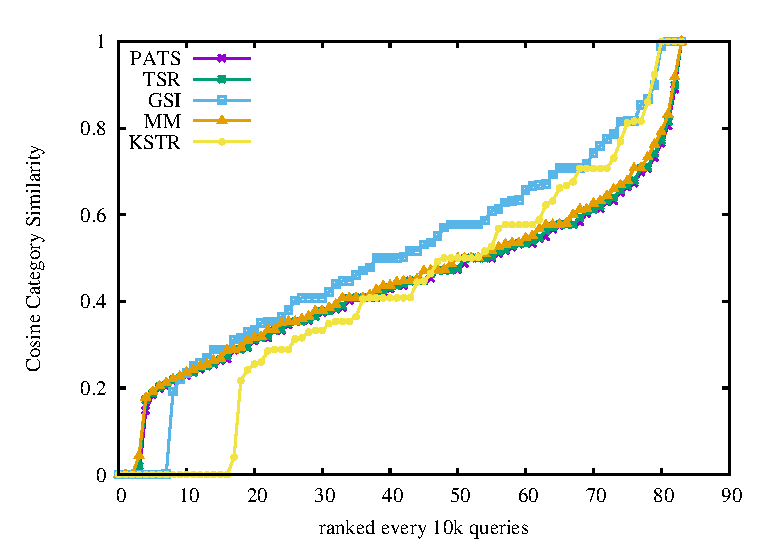
\includegraphics[width=0.33\linewidth]{exp_prediction3_ca.eps}
    }
}
\caption{Average goodness accuracy of recommended travel route at different query region sizes. The yellow line represents our method and shows that KSTR has the good results over the three measurements.}
\label{fig:exp_accuracy}
\end{figure*}

%\textbf{OSScaling model:}
%~\cite{cao2012keyword} outputs the travel routes based on the user’s interests, which is calculated by the Markov model P(lt|lt−1). The most chosen landmark, given the current landmark, is always recommended. This model considers the user’s current location but does not consider the user’s interest.

%\textbf{Markov-Topic model:}
%~\cite{kurashima2010travel} outputs the next route based on the user’s current location and interest, which is calculated by combining the Markov model and the topic model using the unigram rescaling technique.

\noindent\textbf{Pattern aware trajectory search (PATS):}
Only consider the sum of the POI attractiveness score. Different to the Multinomial model, \cite{PATS} consider the mobility transition among POI pairs.

\noindent\textbf{Time-sensitive routes (TSR):}
Only consider the visiting time score of routes. The arrival time of the POIs in the recommendation best fits the extracted proper visiting time.

\noindent\textbf{Geo-social influenced routes (GSI):}
Only consider the geo-social influence score of \cite{ytwen2014}. The route consists of POIs visited by geo-social influential users in social network.

\noindent\textbf{Multinomial model (MM):} 
This is the naive method that outputs the travel routes based on all three features. Routes are ranked by the summation of the feature scores. % r!!! evised

\noindent\textbf{Keyword-aware skyline route (KSTR):}
\textit{KSTR} outputs diverse Skyline routes based on both POI and user factors.

Unfortunately, raw LBSN data provide no ground truth to verify the acceptance of the recommended travel route suggestions. Therefore,
we studied the ``appropriateness'' of the recommended travel routes as a route prediction progress under different spare time conditions. We used the data shown in Table IV for training and testing the model. For each dataset, the test data were created by collecting the last travel sequence of the top-10\% of users (ranked by route count) in the most recent $30$\% time periods. The training dataset consisted of the set of travel sequences excluding the testing data part. To be exact, the number of training data (the number of test data) used in this experiment is slightly larger than the number of testing data since users with multiple travel sequences only keep the last sequence. 
% In order to evaluate the goodness of our method of adding query points into existing trajectories, we remove one ROI from each existing trajectory as a query point and then use our method to aggregate the removed ROI back into the trajectories. We call hit if the order of ROIs in the trajectories after aggregating the query point by our method is the same as the original trajectory order, as it indicates that the order is appropriate because there exists history trajectories that someone visited the ROI in the same order. The hit rate of our method in this experiment is about 69\%.

\subsubsection{Comparison of route prediction accuracy}
We measured the difference between the generated routes and each test sequence. Three goodness functions are applied as the evaluation metrics.

\noindent\textbf{Edit distance:} 
The edit distance measures the distance between two sequences in terms of the minimum number of edit operations required to transform one sequence into the other~\cite{kurashima2010travel}. The allowable edit operations are: insert into a sequence, delete from a sequence, and replace one landmark with another.

\noindent\textbf{Geographical region cover ratio:}
The test route and recommended route both can be bounded by a geographical box. The ratio of the overlapped region to the testing route region.

\noindent\textbf{Category similarity:}
To consider the closeness of user interest, we compute the cosine similarity of the categories between two routes, which is \textit{\# of overlapped category} / $\sqrt{\textit{\# of category1}\cdot\textit{\# of category2} }$.

We compared our \textit{KSTR} model with the other models: multinomial model, pattern aware trajectory search, time-sensitive and geo-social influenced routes. Figure~\ref{fig:exp_accuracy} shows the performance of each model among the three measures. We can find that the proposed \textit{KSTR} model offers the lowest edit distance, which represents the highest prediction accuracy. On the other hand, considering the measure of region cover ratio and category similarity, the multinomial model has better performance than ours. The results show that the proposed \textit{KSTR} is effective and beats other baselines and state-of-the-art methods in terms of route prediction accuracy. % !!! add ore descriptions We also tested the statistical significance of the difference between the average edit distances of the proposed and the baselines using the Wilcoxon signed-rank test. For each region, bandwidth, and spare time condition, the result of the Wilcoxon signed-rank test is p < 0.05 (two-sided test).

% \subsubsection{Running time comparison} \label{sec:exp_run_time}

\subsection{Examples of Route Recommendation: }
As a result, we implemented our proposed methods and constructed a web-based travel route recommender system. One example of recommended routes by the system is show.
\vspace{-1.5mm}

\begin{figure}[h]
\centering
\includegraphics[width=\linewidth]{exp_example2.eps}
\vspace{-7mm}
\caption{Examples of KSTR routes in Kaohsiung.}
\label{fig:example1} % 一定要在 caption 之後
\end{figure}

\vspace{-1.5mm}

Figure~\ref{fig:example1} shows the recommendation examples when the user gives a geographical region of Kaohsiung on the map interface and specifies a one day tour and  keywords [``Si Zih Bay'' ``Cuisine'']. The system provides five different trip plans. Note that, unlike ranking, the ordering of skyline results does not reflect relevance. \textit{Route \#4} is visualized on the map interface and each icon on the map represents a POI. Besides the specific region ``Si Zhi Bay'', ``Guo Ji meat dumpling'' and ``ShanMinng TeaShop'' are perfectly associated with the keyword ``Cuisine''. And we can see the route with the best visiting time suggestions.

\vspace{-3mm}

\nocite{PGT2014,Ye2012,WSDM2012finding,VLDB2010,ICDE2013,SDM2011,SIGMOD2010,rendle2010factorizing,WWW2009,ye2011exploiting,photo2trip,BBS,yuan2014graph,ge2010energy,MM2010,cao2012keyword,zheng2015approximate,SIGKDD07_TPM}

\section{Conclusion}
\vspace{-1mm}
In this paper, we study the travel route recommendation problem. We have developed a \textit{KSTR} framework to suggest travel trajectories with a specific range and a set of user preference keywords. These travel trajectories are related to all or partial user preference keywords, and are recommended based on (i) the attractiveness of the POIs it passed, (ii) visiting the POIs at their corresponding proper arrival time, and (iii) the route generated by influential users. We propose a novel keyword extraction module to identify the semantic meaning and match measurement of routes, and design a route reconstruction algorithm to aggregate trajectory segments into travel routes in accordance with query range and time period. We leverage score functions for the three aforementioned features and adapt Skyline search for travel route recommendation instead of the traditional top-$K$ system. The experimental results demonstrate that \textit{KSTR} is able to retrieve travel routes that are interesting for users and outperforms baseline algorithms in terms of effectiveness and efficiency.
\vspace{-1mm}
% conference papers do not normally have an appendix

% use section* for acknowledgement
\section*{Acknowledgment}
Wen and Peng were supported in part by MOST Taiwan, Project No. 102-2221-E-009 -171 -MY3  and 104-2221-E-009 -138 -MY2, by Academic Sinica Theme project, Project No. AS-102-TPA06. Hwang and Yeo were supported by ICT R\&D program of MSIP/IITP [B0101-15-0307] and Microsoft Research.

\vspace{-1mm}

\IEEEpeerreviewmaketitle
\scriptsize
\bibliographystyle{IEEEtran}
\bibliography{reference}

% that's all folks
\end{document}


